\section[Windows Internal]{Windows Internal}

In this section, we introduce some key points of the Windows operating system.
These key points are executive objects, the kernel pool, the global list, and
debug symbols used by Windows.

\subsection[Executive Objects]{Executive Objects}

Windows executive objects are kernel structures allocated and prepended with
various headers. Only some kernel structures are allocated this way, a common
list of executive objects often used for forensics is in the Table
\ref{tab:execobj}. Executive objects must have a header called
\texttt{\_OBJECT\_HEADER}, but it can have other optional headers data.
Forensics tools often use these headers' data to get some general information
about the allocation. Below we discuss some kernel structures and their roles
in the Windows operating system.

\begin{table}[t]
\centering
\begin{tabular}{ll}
\hline
  Object        & Structure                         \\ \hline
  Process       & \texttt{\_EPROCESS}               \\
  Thread        & \texttt{\_ETHREAD}                \\
  File          & \texttt{\_FILE\_OBJECT}           \\
  Driver        & \texttt{\_DRIVER\_OBJECT}         \\
  Mutex         & \texttt{\_KMUTANT}                \\
  Token         & \texttt{\_TOKEN}                  \\
  Symbolic link & \texttt{\_OBJECT\_SYMBOLIC\_LINK} \\
  Type          & \texttt{\_OBJECT\_TYPE}           \\
  Key           & \texttt{\_CM\_HIVE}               \\
\end{tabular}
\caption{Comprehensive list of executive objects}
\label{tab:execobj}
\end{table}

\subsubsection[EPROCESS]{EPROCESS}

\texttt{\_EPROCESS} is a structure to manage the running process. This
structure contains the process id, the parent process id, the memory map for
the process, the process environment block, the pointer to list of loaded
modules, the pointer to list of threads created by the process and other
information related to the process.  This structure is also a node in a
circular doubly linked list of processes.

The memory map is the list of sections inside a process address space, and
these are code, data, heap, libraries. It is represented as a self-balancing
tree where each node contains the address, size, and operations
(Read/Write/Execution) allowed in the region. This tree is often called as
\textit{Vad tree}, and the root of the tree is the \texttt{VadRoot} member in
\texttt{\_EPROCESS}.

The process environment block contains the information to the process, such as
the image base address, the heap pointer. This block resides in the user space
memory, so the kernel process can not read this information. However, the
pointer to the address of the block is the \texttt{PEB} member, and if we map
this address into the kernel space, we can access this information.

\begin{lstlisting}[language=windbg,caption=\texttt{\_EPROCESS} in Windows 7,float,floatplacement=H]
kd> dt _EPROCESS
nt!_EPROCESS
   +0x168 CreateTime       : _LARGE_INTEGER
   +0x170 ExitTime         : _LARGE_INTEGER
   +0x180 UniqueProcessId  : Ptr64 Void
   +0x188 ActiveProcessLinks : _LIST_ENTRY
   +0x238 PhysicalVadRoot  : Ptr64 _MM_AVL_TABLE
   +0x258 Win32Process     : Ptr64 Void
   +0x290 InheritedFromUniqueProcessId : Ptr64 Void
   +0x2e0 ImageFileName    : [15] UChar
   +0x308 ThreadListHead   : _LIST_ENTRY
   +0x328 ActiveThreads    : Uint4B
   +0x338 Peb              : Ptr64 _PEB
   +0x448 VadRoot          : _MM_AVL_TABLE
\end{lstlisting}

\begin{lstlisting}[language=windbg,caption=\texttt{\_PEB} in Windows 7,float,floatplacement=H]
kd> dt _PEB
nt!_PEB
   +0x002 BeingDebugged    : UChar
   +0x003 ImageUsesLargePages : Pos 0, 1 Bit
   +0x003 IsProtectedProcess : Pos 1, 1 Bit
   +0x003 IsLegacyProcess  : Pos 2, 1 Bit
   +0x003 IsImageDynamicallyRelocated : Pos 3, 1 Bit
   +0x003 SkipPatchingUser32Forwarders : Pos 4, 1 Bit
   +0x008 Mutant           : Ptr64 Void
   +0x010 ImageBaseAddress : Ptr64 Void
   +0x018 Ldr              : Ptr64 _PEB_LDR_DATA
   +0x030 ProcessHeap      : Ptr64 Void
   +0x050 CrossProcessFlags : Uint4B
   +0x0c8 HeapSegmentReserve : Uint8B
   +0x0d0 HeapSegmentCommit : Uint8B
   +0x0d8 HeapDeCommitTotalFreeThreshold : Uint8B
   +0x0e0 HeapDeCommitFreeBlockThreshold : Uint8B
   +0x0e8 NumberOfHeaps    : Uint4B
   +0x0ec MaximumNumberOfHeaps : Uint4B
   +0x0f0 ProcessHeaps     : Ptr64 Ptr64 Void
\end{lstlisting}

\subsubsection[ETHREAD]{ETHREAD}

\texttt{\_ETHREAD} is a structure used to manage threads. This structure
contains the process id, the thread id, the pointer to the owner
\texttt{\_EPROCESS}, current thread state, threads flags. This structure is
also a node in a circular doubly linked list of threads. The status of the
thread can tell whether the thread is initilized, ready, running, or waiting.
The thread waiting reason can also be found in this structure. Thread's flags
indicate the thread to be terminated, dead, hided from debugger, impersonating,
a system thread.

\begin{lstlisting}[language=windbg,caption=\texttt{\_ETHREAD} in Windows 7,float,floatplacement=H]
kd> dt _ETHREAD
nt!_ETHREAD
   +0x000 Tcb              : _KTHREAD
      +0x164 State            : UChar
      +0x210 Process          : Ptr64 _KPROCESS or _EPROCESS
      +0x26b WaitReason       : UChar
   +0x360 CreateTime       : _LARGE_INTEGER
   +0x368 ExitTime         : _LARGE_INTEGER
   +0x378 ExitStatus       : Int4B
   +0x388 StartAddress     : Ptr64 Void
   +0x3b0 Cid              : _CLIENT_ID
      +0x000 UniqueProcess    : Ptr64 Void
      +0x008 UniqueThread     : Ptr64 Void
   +0x420 ThreadListEntry  : _LIST_ENTRY
   +0x448 CrossThreadFlags : Uint4B
\end{lstlisting}

\subsubsection[KMUTANT]{KMUTANT}

\textit{Mutant} is the way Windows name \textit{mutex}, a lock to prevent
multiple threads accessing the same time, and represented using a
\texttt{\_KMUTANT}.  A mutant has a pointer to the thread owning the mutant.

\begin{lstlisting}[language=windbg,caption=\texttt{\_KMUTANT} in Windows 7,float,floatplacement=H]
kd> dt _KMUTANT
nt!_KMUTANT
   +0x018 MutantListEntry  : _LIST_ENTRY
   +0x028 OwnerThread      : Ptr64 _KTHREAD
\end{lstlisting}

\subsubsection[DRIVER\_OBJECT]{DRIVER\_OBJECT}

Every driver loaded and running will be represented with a type of
\texttt{\_DRIVER\_OBJECT}.  This structure contains a pointer to the underlying
device and functions related to this driver. Functions related to the driver
are \textit{init}, \textit{unload} and 28 major functions.

\begin{lstlisting}[language=windbg,caption=\texttt{\_DRIVER\_OBJECT} in Windows 7,float,floatplacement=H]
kd> dt _DRIVER_OBJECT
nt!_DRIVER_OBJECT
   +0x000 Type             : Int2B
   +0x002 Size             : Int2B
   +0x008 DeviceObject     : Ptr64 _DEVICE_OBJECT
   +0x018 DriverStart      : Ptr64 Void
   +0x020 DriverSize       : Uint4B
   +0x028 DriverSection    : Ptr64 Void
   +0x030 DriverExtension  : Ptr64 _DRIVER_EXTENSION
   +0x038 DriverName       : _UNICODE_STRING
   +0x048 HardwareDatabase : Ptr64 _UNICODE_STRING
   +0x050 FastIoDispatch   : Ptr64 _FAST_IO_DISPATCH
   +0x058 DriverInit       : Ptr64     long
   +0x060 DriverStartIo    : Ptr64     void
   +0x068 DriverUnload     : Ptr64     void
   +0x070 MajorFunction    : [28] Ptr64     long
\end{lstlisting}

\subsection[Other kernel structures]{Other kernel structures}

\subsubsection[LDR\_DATA\_TABLE\_ENTRY]{LDR\_DATA\_TABLE\_ENTRY}

Windows tracks \textit{modules}, dynamically loaded library, loaded in each
process by a structure called \texttt{\_LDR\_DATA\_TABLE\_ENTRY}, this
structure is a node in three different circular linked lists, \textit{in load}
list, \textit{in memory} list, and \textit{in initilization} list. This
structure contains the base address, the entry point address, the size, the
name of the module, and the number of processes loaded. The kernel module is
tracked using \texttt{\_KLDR\_DATA\_TABLE\_ENTRY}, which has some small
differences, but the layout is almost the same.

\begin{lstlisting}[language=windbg,caption=\texttt{\_LDR\_DATA\_TABLE\_ENTRY} in Windows 7,float,floatplacement=H]
kd> dt _LDR_DATA_TABLE_ENTRY
nt!_LDR_DATA_TABLE_ENTRY
   +0x000 InLoadOrderLinks : _LIST_ENTRY
   +0x010 InMemoryOrderLinks : _LIST_ENTRY
   +0x020 InInitializationOrderLinks : _LIST_ENTRY
   +0x030 DllBase          : Ptr64 Void
   +0x038 EntryPoint       : Ptr64 Void
   +0x040 SizeOfImage      : Uint4B
   +0x048 FullDllName      : _UNICODE_STRING
   +0x058 BaseDllName      : _UNICODE_STRING
   +0x06c LoadCount        : Uint2B
\end{lstlisting}

\subsection[Kernel pool]{Kernel pool}
\label{sec:pool}

The kernel pool is the way Windows named the kernel heap for dynamic memory
allocation. There are many pools, each with different types, and the system
memory space has specific ranges for these pools. However, there are two main
types of pool, the paged pool, and non-paged pool. The paged pool can be paged
out to disk while the non-paged pool is always in memory. The non-paged pool is
mostly used for system structures where the allocation must always be in memory
for fast accessing. Allocation in a pool has a pool header data prepended.  The
pool header, of type \texttt{\_POOL\_HEADER}, contains the size of the
allocation, the size of the previous allocation, the type of the pool
allocated, and a four-byte tag. For convenience, we call an allocation a
\textbf{block}.  The size in the header is a multiplier of 16 in 64-bit
systems.  The type of pool is an enumeration, and it should match the pool type
where the block was allocated. The four-byte tag is a value provided when
allocate the block using legacy Windows API such as
\texttt{ExAllocatePoolWithTag}. In Figure \ref{fig:pooltag}, we can see how the
pool allocation works.

\begin{figure}[h]
  \centering
  \caption{Pool Allocation}
  \label{fig:pooltag}
  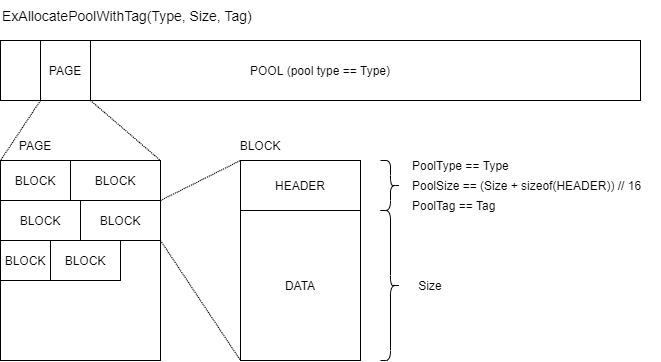
\includegraphics[scale=0.7]{images/pooltag.png}
\end{figure}

The pool that is relevant to the kernel data is called the non-paged pool. This
pool's pages are never paged out to disk and contain many executive objects.
The header of blocks allocated inside this pool will have the type value equal
to 2. Kernel objects are allocated inside this pool with a tag hard-coded
inside the kernel code. Their tags and the structure are described in the Table
\ref{tab:pooltag}.

\begin{lstlisting}[language=windbg,caption=\texttt{\_POOL\_HEADER} in Windows 64-bit,float,floatplacement=H]
kd> dt _POOL_HEADER
nt!_POOL_HEADER
   +0x000 PreviousSize     : Pos 0, 8 Bits
   +0x000 PoolIndex        : Pos 8, 8 Bits
   +0x000 BlockSize        : Pos 16, 8 Bits
   +0x000 PoolType         : Pos 24, 8 Bits
   +0x004 PoolTag          : Uint4B
\end{lstlisting}

\subsection[Global list]{Global list}

Windows has several global lists to control the systems, the head (pointer) of
these lists is saved inside global variables in the kernel. For processes,
Windows has two circular doubly linked lists, indexed by
\texttt{PsActiveProcessHead}, \texttt{KiProcessListHead}.  There is also a
handle table list, \texttt{HandleTableListHead}, where each handle has a
pointer to \texttt{\_EPROCESS}. Kernel modules are also stored inside the
\texttt{PsLoadedModuleList}.

\subsection[Debug symbols]{Debug symbols}

The Windows source code is not publicly available, however Windows distributes
debug symbols for researching purposes. These debug symbols contains the offset
to global variables, functions and structure layout. The symbols are compressed
into a file called program database, or \textit{PDB}, with the extension
\texttt{.pdb}. The instruction to extract the file is limited described
\cite{microsoft-pdb}, but public works have been done and parsers are
available.

A PDB file is unique to one specific version of a kernel module. The PDB file
for the main kernel module is named \texttt{ntkrnlmp.pdb} for the kernel module
\texttt{C:\textbackslash \textbackslash Windows \textbackslash System32
\textbackslash ntoskrnl.exe}. The binary \texttt{ntoskrnl.exe} is different
across Windows updates. Downloading a specific PDB file for the kernel requires
the module's id, \textit{GUID}, and \textit{age}. GUID and age are parsed from
the binary in the RSDS section of a PE file \footnote{Executable file in
Windows OS}. In the same Windows version, specifically the Windows minor
version, structures layout are the same, but addresses to global variables and
functions are different.  Across different Windows' major version, huge changes
in structure layout, new functions and variables were introduced, and old ones
were removed. This is why downloading the correct PDB file for the current
machine is better than hardcoding the addresses, and members offset.

The Microsoft PDB server hosting the PDB files is located at
\url{https://msdl.microsoft.com/download/symbols}. To download the main kernel
module, we need to build the request URL as defined in Listing
\ref{lst:downloadpdb}. After that, parsing the PDB can be done using public
libraries, PDB parser by Brendan\cite{pdbparse} or PDB by Will
Glynn\cite{pdbrust}.

\begin{lstlisting}[language=cpp,caption=Download PDB file,label={lst:downloadpdb},float,floatplacement=H]
const string root_url = "https://msdl.microsoft.com/download/symbols/";
const string pdb_name = "ntkrnlmp.pdb";
const string guid = "XXXX";
const string age = "01";

const string download_url = root_url + pdb_name + "/"
                          + guid + age + "/"
                          + pdb_name;
\end{lstlisting}
